\chapter{Diversidad de los organismos unicelulares}\label{ch:b2:unicellular-diversity}

Una gota de agua de charca bajo el microscopio contiene una célula verde
que rema con dos flagelos, un ciliado con forma de zapatilla que barre
bacterias hacia su citofaringe, una diatomea vítrea que se desliza por el
portaobjetos y, demasiado pequeñas para verlas bien, mil bacterias. Cada
una es una sola célula y cada una es un organismo completo: se alimenta,
se mueve, percibe, crece, se reproduce y muere como una célula aislada.
La mayor parte del mundo vivo ha sido siempre así. Este capítulo trata el
\omterm{def:b2:unicellular-diversity:unicellular}{organismo unicelular} como un problema de diseño --- lo que una célula
puede y no puede hacer --- y repasa las respuestas que han encontrado
\omterm{def:b2:unicellular-diversity:prokaryote}{procariotas} y eucariotas, hasta el punto en que las células empiezan a
permanecer juntas.

\section{Una célula, todas las funciones}

\begin{definition}[Unicelular, colonial, pluricelular]\label{def:b2:unicellular-diversity:unicellular}
Un organismo es \emph{unicelular}\index{organismo unicelular} cuando una
sola célula realiza todas las funciones de la vida --- nutrición,
intercambios, movimiento, reproducción --- y vive por sí misma. Es
\emph{colonial}\index{organismo colonial} cuando células de un mismo tipo
permanecen unidas tras dividirse, pero cada una sigue siendo capaz de
vivir sola si se la separa. Es \emph{pluricelular}\index{organismo pluricelular}
cuando sus células son de varios tipos, dependen unas de otras y solo
unas pocas (la línea germinal) dejan descendencia. Son unicelulares
todas las arqueas, casi todas las bacterias y la mayoría de los linajes
de eucariotas; el nombre informal de \emph{\omterm{def:b2:unicellular-diversity:protist}{protista}} abarca los
eucariotas unicelulares, que no forman un grupo sino muchos.
\end{definition}

\begin{example}[Seis habitantes de una gota]\label{ex:b2:unicellular-diversity:drop}
\emph{Escherichia coli}, un bastón de \qty{2}{\micro m} de largo, nada
con un penacho de flagelos y se divide cada veinte minutos si tiene
alimento. \emph{Chlamydomonas}, un alga verde de \qty{10}{\micro m} de
diámetro, rema con dos flagelos hacia la luz, que detecta con un
estigma. \emph{Paramecium}, un ciliado de \qty{200}{\micro m}, está
cubierto de miles de cilios, se alimenta por una citofaringe y achica el
agua con dos \omterm{prop:b2:unicellular-diversity:osmoregulation}{vacuolas contráctiles}. Una diatomea vive en un caparazón de
sílice de dos piezas, ornamentado con poros. \emph{Amoeba} fluye
emitiendo pseudópodos y engloba lo que encuentra. Una célula de levadura
forma una hija en yema sobre su costado. Seis respuestas, de tamaño y
maquinaria muy distintos, a un mismo problema.
\end{example}

\begin{omfigure}
\begin{tikzpicture}[x=1.9cm]
  % log scale from 0.1 um to 100 mm : position = log10(size in um) + 1
  \draw[thick] (0,0) -- (6,0);
  \foreach \p/\l in {0/{\qty{0.1}{\micro m}},1/{\qty{1}{\micro m}},2/{\qty{10}{\micro m}},3/{\qty{100}{\micro m}},4/{\qty{1}{mm}},5/{\qty{10}{mm}},6/{\qty{100}{mm}}}
    \draw (\p,0.12) -- (\p,-0.12) node[below, font=\scriptsize] {\l};
  \foreach \p/\c/\l in {0.5/omDef/micoplasma, 1.3/omDef/{\emph{E.~coli}}, 1.7/omDef/levadura, 2.0/omProp/{\emph{Chlamydomonas}}, 2.7/omProp/diatomeas, 3.3/omProp/{\emph{Paramecium}}, 3.65/omProp/{\emph{Amoeba proteus}}, 3.9/omThm/{\emph{Thiomargarita} (una bacteria)}, 5.7/omProp/{\emph{Acetabularia}}}
    { \fill[\c] (\p,0) circle (0.05); \node[rotate=60, anchor=west, font=\scriptsize, \c, inner sep=1pt] at (\p,0.12) {\l}; }
  \node[font=\scriptsize, anchor=north] at (3,-0.55) {tamaño celular (escala logarítmica)};
\end{tikzpicture}

{\small El tamaño de los \omterm{def:b2:unicellular-diversity:unicellular}{organismos unicelulares} abarca cinco órdenes de
magnitud. Los \omterm{def:b2:unicellular-diversity:prokaryote}{procariotas} (azul) se agrupan en torno a un micrómetro; las
células eucariotas (naranja) son de diez a cien veces mayores; las
células aisladas más grandes --- una bacteria gigante del azufre, el alga
\emph{Acetabularia} --- son excepciones que el texto explica.}
\end{omfigure}

\begin{proposition}[Superficie, volumen y el límite del tamaño]\label{prop:b2:unicellular-diversity:surface}
\index{relación superficie/volumen}
Una célula intercambia con su entorno a través de su superficie y
consume en proporción a su volumen. Para una esfera de radio $r$, la
\emph{\omterm{prop:b2:unicellular-diversity:surface}{relación superficie/volumen}} es
\[
\frac{S}{V} = \frac{4\pi r^2}{\tfrac{4}{3}\pi r^3} = \frac{3}{r},
\]
de modo que duplicar el radio reduce a la mitad la superficie disponible
por unidad de citoplasma. Una célula que depende de la difusión a través
de su membrana para abastecer su interior no puede, por tanto, crecer
indefinidamente: a partir de cierto radio el aporte a través de la
superficie ya no cubre la demanda del volumen. La misma ley explica por
qué las células pequeñas son las más activas metabólicamente por gramo, y
por qué las células grandes son aplanadas, alargadas, vacuolizadas o
están llenas de membranas internas.
\end{proposition}

\begin{theorem}[Tiempo para difundir una distancia]\label{thm:b2:unicellular-diversity:diffusion}
\index{tiempo de difusión}
Una molécula de coeficiente de difusión $D$ se desplaza a pasos
aleatorios; al cabo de un tiempo $t$ su desplazamiento cuadrático medio
a lo largo de un eje es $\langle x^2\rangle = 2Dt$. El tiempo necesario
para recorrer una distancia $x$ solo por difusión es, por tanto,
\[
t \approx \frac{x^2}{2D},
\]
que crece con el \emph{cuadrado} de la distancia. Con
$D \approx \qty{1e-9}{m^2/s}$ para una molécula pequeña en agua, cruzar
una bacteria (\qty{1}{\micro m}) lleva medio milisegundo; cruzar una
célula de \qty{1}{mm} llevaría ocho minutos, y un metro, dieciséis
años.
\end{theorem}
\begin{proof}
Supóngase que la molécula da pasos de longitud $\ell$ al azar hacia la
izquierda o la derecha cada $\tau$ segundos. Tras $n$ pasos su
desplazamiento es $x = \sum_i \varepsilon_i \ell$ con $\varepsilon_i = \pm 1$
independientes, de modo que $\langle x\rangle = 0$ y $\langle x^2\rangle =
\sum_i \langle\varepsilon_i^2\rangle \ell^2 = n\ell^2$ (los términos
cruzados se anulan en promedio). Con $n = t/\tau$ esto da $\langle x^2\rangle
= (\ell^2/\tau)\,t$, y escribiendo $D = \ell^2/2\tau$ se obtiene
$\langle x^2\rangle = 2Dt$. Igualando $\langle x^2\rangle = x^2$ se
obtiene el tiempo.
\end{proof}

\begin{theorem}[Aporte difusivo a una célula esférica]\label{thm:b2:unicellular-diversity:supply}
\index{captación limitada por difusión}
Una célula esférica de radio $r_0$ que absorbe toda molécula de un
soluto que alcanza su superficie, en un medio cuya concentración lejos
de ella es $c_\infty$, recibe en régimen estacionario un flujo (moléculas
por segundo) de
\[
J = 4\pi D r_0\, c_\infty .
\]
El aporte solo crece con $r_0$, mientras que la demanda crece con
$r_0^3$: más allá de cierto radio, una célula alimentada por difusión
pasa hambre.
\end{theorem}
\begin{proof}
En régimen estacionario el número de moléculas que atraviesan por
segundo cada esfera de radio $r > r_0$ es el mismo, $J = 4\pi r^2 D\,
(\mathrm{d}c/\mathrm{d}r)$ (ley de Fick, con el flujo dirigido hacia dentro).
Así, $r^2\,\mathrm{d}c/\mathrm{d}r = J/4\pi D$ es constante; integrando
desde $r_0$, donde $c = 0$, hasta el infinito, donde $c = c_\infty$:
$c_\infty = (J/4\pi D)\int_{r_0}^{\infty} r^{-2}\,\mathrm{d}r =
J/(4\pi D r_0)$, de donde $J = 4\pi D r_0 c_\infty$.
\end{proof}

\begin{example}[¿Qué tamaño puede tener una célula alimentada por difusión?]\label{ex:b2:unicellular-diversity:howbig}
Una célula aerobia consume oxígeno a razón de unos $q = \qty{0.02}{mol/m^3/s}$
de citoplasma (un ritmo intenso). Su demanda es $q \cdot \tfrac{4}{3}\pi
r_0^3$; el aporte desde agua saturada de aire ($c_\infty =
\qty{0.25}{mol/m^3}$, $D = \qty{2e-9}{m^2/s}$) es $4\pi D r_0
c_\infty$. Igualando, $r_0^2 = 3Dc_\infty/q = 3\times 2\times 10^{-9}
\times 0.25/0.02 = \qty{7.5e-8}{m^2}$, luego $r_0 \approx
\qty{270}{\micro m}$. Las células activas reales quedan muy por debajo,
porque el oxígeno también debe difundir \emph{dentro} de ellas; la
bacteria del azufre \emph{Thiomargarita}, de \qty{750}{\micro m}, sortea
el límite siendo casi por completo una vacuola, con el citoplasma
reducido a una fina capa de unos pocos micrómetros de espesor.
\end{example}

\begin{omfigure}
\begin{tikzpicture}
\begin{axis}[
  width=0.8\linewidth, height=6.2cm,
  axis x line=bottom, axis y line=left,
  xmode=log, ymode=log,
  xmin=0.3, xmax=1000, ymin=1e-6, ymax=1e4,
  xlabel={radio celular (\unit{\micro m})}, ylabel={moléculas por segundo (relativo)},
  xlabel style={font=\small, at={(axis description cs:0.5,-0.1)}, anchor=north},
  ylabel style={font=\small},
  tick label style={font=\small},
  legend style={font=\small, at={(0.03,0.97)}, anchor=north west, draw=none},
  clip=false,
]
\addplot[very thick, omDef, domain=0.3:1000, samples=40] {x/10};
\addlegendentry{aporte por difusión, $\propto r$}
\addplot[very thick, omThm, domain=0.3:1000, samples=40] {(x/10)^3/1000*1.0};
\addlegendentry{demanda del citoplasma, $\propto r^3$}
\draw[dashed, gray] (axis cs:270,1e-6) -- (axis cs:270,27);
\node[font=\scriptsize, anchor=west] at (axis cs:300,3e-4) {radio de inanición};
\end{axis}
\end{tikzpicture}

{\small El aporte a través de la superficie crece con $r$, la demanda con
$r^3$ (ejes logarítmicos). Donde las rectas se cruzan, una célula
alimentada solo por difusión ya no puede abastecer su interior; para
una célula aerobia activa el cruce se sitúa en torno a unos cientos de
micrómetros.}
\end{omfigure}

\section{Diversidad de los procariotas}

\begin{definition}[La célula procariota]\label{def:b2:unicellular-diversity:prokaryote}
Un \emph{procariota}\index{procariota} (las bacterias y las arqueas, dos
dominios tan distintos entre sí como cualquiera de ellos lo es de
nosotros) es una célula sin núcleo ni orgánulos delimitados por
membrana: un único cromosoma circular en un \emph{nucleoide}\index{nucleoide},
a menudo con pequeños círculos adicionales llamados
\emph{plásmidos}\index{plásmido}, ribosomas libres en un citoplasma de
\qtyrange{0.5}{2}{\micro m}, una membrana plasmática que lleva las
cadenas respiratorias o fotosintéticas, y una
\emph{pared celular}\index{pared celular!bacteriana} rígida que resiste
la turgencia de un citoplasma varios bares por encima de su entorno. Las
formas son pocas y tienen nombre: \emph{coco} (esfera), \emph{bacilo}
(bastón), \emph{espirilo} y \emph{espiroqueta} (hélices), \emph{vibrión}
(coma); tras dividirse, las células pueden quedar en parejas, cadenas,
tétradas o racimos.
\end{definition}

\begin{proposition}[Dos envolturas: grampositivas y gramnegativas]\label{prop:b2:unicellular-diversity:gram}
\index{tinción de Gram}\index{peptidoglucano}
La pared bacteriana está hecha de \emph{peptidoglucano}, cadenas de dos
azúcares alternados unidas por péptidos cortos en una única molécula
gigante que rodea la célula. Las bacterias \emph{grampositivas} tienen
una capa gruesa (\qtyrange{20}{80}{nm}) por fuera de una sola membrana
y retienen el cristal violeta de la \omterm{prop:b2:unicellular-diversity:gram}{tinción de Gram}; las bacterias
\emph{gramnegativas} tienen una capa delgada (unos pocos nanómetros)
intercalada entre la membrana plasmática y una \emph{membrana externa}
cuya hoja exterior está formada por lipopolisacárido, y pierden el
colorante. La membrana externa, perforada por porinas, es una segunda
barrera: impide el paso de muchos antibióticos y detergentes, y por eso
las infecciones por gramnegativas son más difíciles de tratar. Las
arqueas no tienen ni peptidoglucano ni los lípidos con enlace éster de
todas las demás células: sus membranas están formadas por cadenas
isoprenoides unidas por enlaces éter, que a veces atraviesan toda la
bicapa formando una monocapa, lo que las mantiene estables en ácido
hirviendo.
\end{proposition}

\begin{omfigure}
\begin{tikzpicture}[scale=0.9, every node/.style={font=\scriptsize}]
  % Gram-positive
  \begin{scope}
    \fill[omDef!15] (0,0) rectangle (4,1.6);
    \node at (2,0.4) {citoplasma};
    \fill[omDef!60] (0,1.6) rectangle (4,1.85);
    \node[right] at (4.05,1.72) {membrana plasmática};
    \fill[omProp!50] (0,1.85) rectangle (4,3.0);
    \foreach \y in {2.0,2.25,...,2.85} \draw[omProp!90!black] (0.1,\y) -- (3.9,\y);
    \node[right, align=left] at (4.05,2.45) {peptidoglucano grueso\\(\qtyrange{20}{80}{nm})};
    \node[above, font=\small\bfseries] at (2,3.05) {Grampositiva};
  \end{scope}
  % Gram-negative
  \begin{scope}[xshift=7.6cm]
    \fill[omDef!15] (0,0) rectangle (4,1.6);
    \node at (2,0.4) {citoplasma};
    \fill[omDef!60] (0,1.6) rectangle (4,1.85);
    \node[right] at (4.05,1.72) {membrana plasmática};
    \fill[omProp!50] (0,2.05) rectangle (4,2.25);
    \draw[omProp!90!black] (0.1,2.15) -- (3.9,2.15);
    \node[right] at (4.05,2.15) {peptidoglucano delgado};
    \node at (2,1.95) {periplasma};
    \fill[omThm!50] (0,2.55) rectangle (4,2.85);
    \foreach \x in {0.6,2.0,3.4} \fill[white] (\x-0.12,2.55) rectangle (\x+0.12,2.85);
    \node[right] at (4.05,2.7) {membrana externa con porinas};
    \foreach \x in {0.2,0.5,...,3.9} \draw[omThm!80!black, thick] (\x,2.85) -- (\x,3.1);
    \node[right] at (4.05,3.15) {lipopolisacárido};
    \node[above, font=\small\bfseries] at (2,3.3) {Gramnegativa};
  \end{scope}
\end{tikzpicture}

{\small Las dos envolturas bacterianas en sección. Izquierda: una membrana
bajo una gruesa cubierta de peptidoglucano. Derecha: una capa delgada de
peptidoglucano en el periplasma, entre dos membranas, la externa
salpicada de porinas y recubierta de lipopolisacárido.}
\end{omfigure}

\begin{proposition}[El flagelo bacteriano y la quimiotaxis]\label{prop:b2:unicellular-diversity:flagellum}
\index{flagelo!bacteriano}\index{quimiotaxis}
El \emph{flagelo} bacteriano es un filamento helicoidal rígido de la
proteína flagelina, de \qty{20}{nm} de grosor y varias longitudes
corporales de largo, que hace girar un motor rotatorio anclado en la
envoltura. El motor no funciona con ATP sino con protones que fluyen a
favor del gradiente electroquímico a través de la membrana, a razón de
unos \num{1000} protones por vuelta y hasta \num{300} vueltas por
segundo. En \emph{E.~coli} los distintos flagelos se reúnen en un haz
cuando todos giran en sentido antihorario y empujan la célula en una
\emph{carrera} rectilínea; cuando uno o varios invierten el giro, el haz
se deshace y la célula da una \emph{voltereta} hacia una nueva dirección
aleatoria. La \emph{quimiotaxis} es el sesgo de este paseo aleatorio: la
célula mide si la concentración de un atrayente ha aumentado durante el
último segundo y, en tal caso, suprime las volteretas. Se orienta
comparando el presente con el pasado reciente --- a lo largo de su
trayectoria --- porque a lo largo de su propio
\qty{1}{\micro m} de longitud no hay gradiente medible.
\end{proposition}
\begin{proof}[Evidencia]
Berg y Brown (1972) siguieron células aisladas de \emph{E.~coli} en tres
dimensiones con un microscopio de seguimiento: carreras de alrededor de
un segundo a \qty{20}{\micro m/s}, volteretas de una décima de segundo y,
en un gradiente de serina, carreras más largas gradiente arriba sin que
las carreras gradiente abajo se acortaran. Fijar una célula a un
portaobjetos por un solo flagelo hacía girar todo el cuerpo, lo que
demostró que el motor es rotatorio; las células con el motor desacoplado
de la síntesis de ATP seguían nadando mientras se pudiera imponer un
gradiente de protones, lo que identificó el combustible.
\end{proof}

\begin{omfigure}
\begin{tikzpicture}[every node/.style={font=\scriptsize}]
  % run and tumble path without gradient
  \begin{scope}
    \draw[very thick, omDef] (0,0) -- (1.2,0.5) -- (0.7,1.4) -- (1.9,1.8) -- (2.6,0.9) -- (3.4,1.5) -- (3.0,2.5);
    \foreach \p in {(1.2,0.5),(0.7,1.4),(1.9,1.8),(2.6,0.9),(3.4,1.5)} \fill[omThm] \p circle (0.06);
    \node[align=center] at (1.8,-0.5) {sin gradiente:\\carreras de igual longitud, giros al azar};
  \end{scope}
  \begin{scope}[xshift=6cm]
    \shade[left color=white, right color=omExo!50] (-0.3,-0.2) rectangle (5.2,3.0);
    \draw[very thick, omDef] (0,0.3) -- (0.9,0.8) -- (0.6,1.3) -- (2.4,1.5) -- (2.2,2.2) -- (4.6,2.4);
    \foreach \p in {(0.9,0.8),(0.6,1.3),(2.4,1.5),(2.2,2.2)} \fill[omThm] \p circle (0.06);
    \node[align=center] at (2.4,-0.5) {atrayente creciente hacia la derecha:\\carreras gradiente arriba más largas};
    \node[anchor=south east] at (5.1,2.6) {más atrayente};
  \end{scope}
\end{tikzpicture}

{\small Carreras y volteretas. Izquierda: sin gradiente, la célula
describe un paseo aleatorio, con cada carrera (azul) terminada por una
voltereta (punto rojo). Derecha: cuando el atrayente aumenta a lo largo
de una carrera, se suprimen las volteretas y la carrera se alarga; el
paseo deriva gradiente arriba.}
\end{omfigure}

\begin{example}[Las cianobacterias y el heterocisto]\label{ex:b2:unicellular-diversity:cyanobacteria}
Las cianobacterias son las bacterias que realizan la fotosíntesis como
las plantas, rompiendo el agua y liberando oxígeno en membranas internas
apiladas (los tilacoides, que el cloroplasto heredó de ellas). Muchas
crecen como filamentos de células que comparten una vaina. En
\emph{Anabaena}, cuando se agota el nitrógeno combinado, aproximadamente
una de cada diez células se convierte en un \emph{heterocisto}: desmantela
su fotosistema productor de oxígeno, engrosa su pared frente al oxígeno y
fija el nitrógeno atmosférico con una enzima que el oxígeno destruiría,
exportando glutamina a sus vecinas a cambio de azúcar. Un filamento de
\emph{Anabaena} es un primer esbozo de división del trabajo entre
células.
\end{example}

\begin{omfigure}
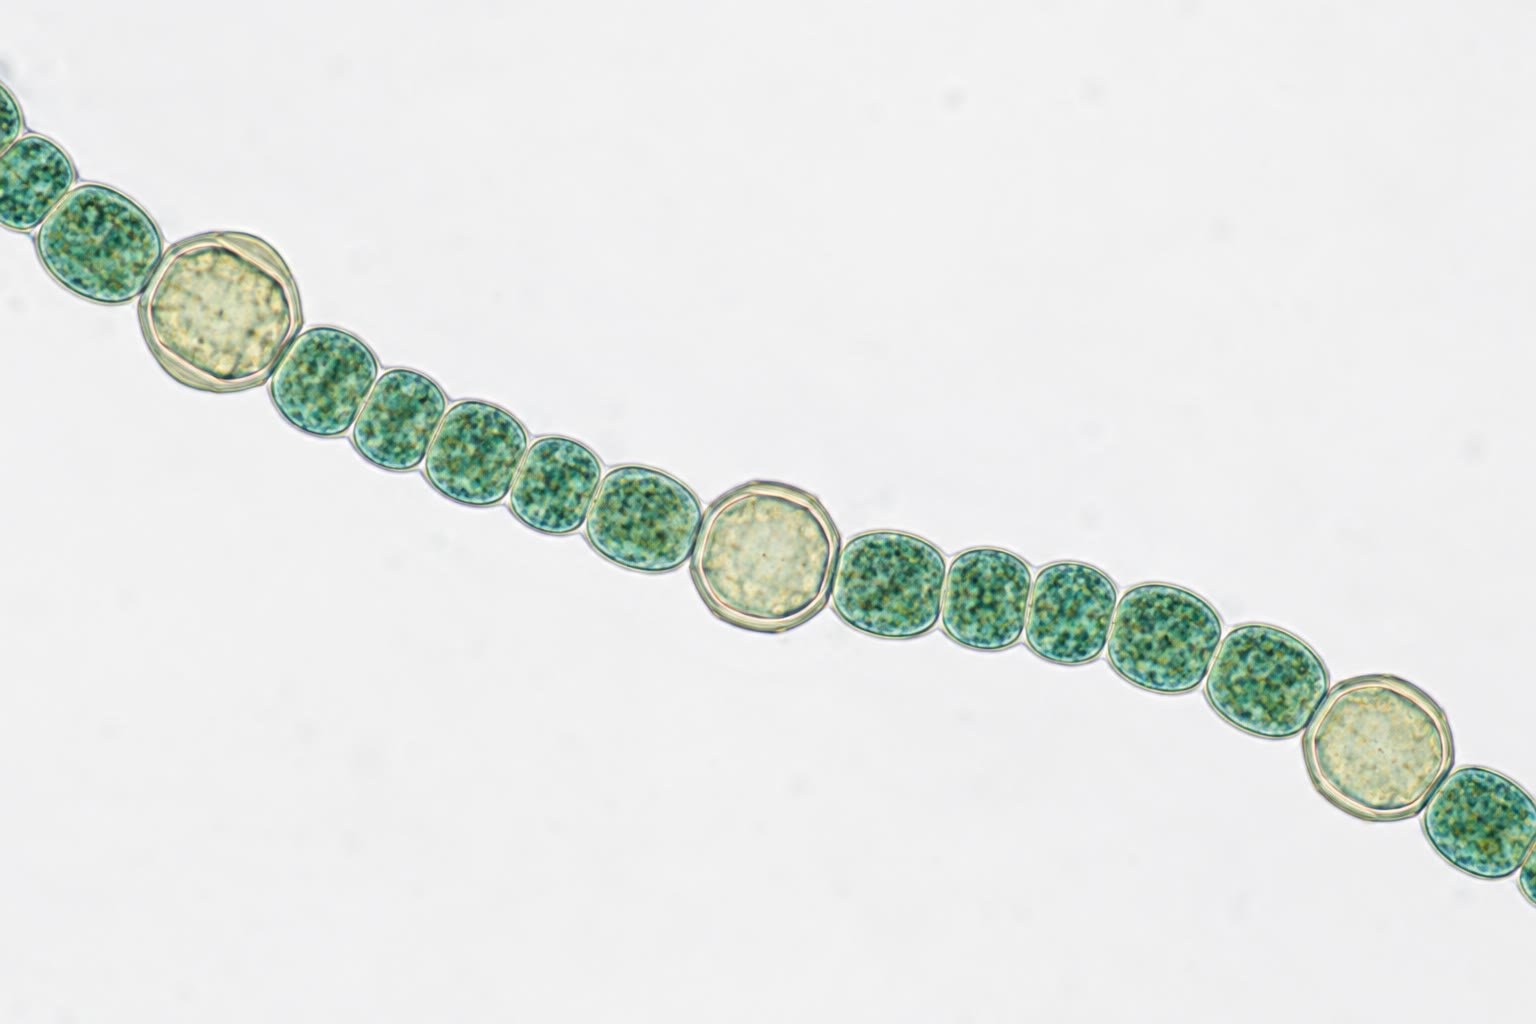
\includegraphics[width=0.62\linewidth]{images/book4/ai/b4-01-anabaena.jpg}

{\small Un filamento de \emph{Anabaena}: una cadena de células verdes
fotosintéticas interrumpida por heterocistos, más grandes y pálidos,
las células que fijan el nitrógeno.}
\end{omfigure}

\begin{remark}[Latencia]\label{rem:b2:unicellular-diversity:spores}
Algunos bacilos grampositivos (\emph{Bacillus}, \emph{Clostridium})
responden a la inanición formando una \emph{endospora}: una copia del
cromosoma envuelta en varias cubiertas deshidratadas, metabólicamente
inerte, resistente a la ebullición, a la radiación y a siglos de sequía,
que germina cuando vuelven las condiciones favorables. Muchos \omterm{def:b2:unicellular-diversity:protist}{protistas}
hacen lo mismo con un \emph{quiste}. La latencia es la otra manera de
sobrevivir a una mala estación, junto a la movilidad.
\end{remark}

\section{Los eucariotas unicelulares}

\begin{definition}[Protistas: un grado, no un grupo]\label{def:b2:unicellular-diversity:protist}
Los \emph{protistas}\index{protista} son los eucariotas que no son ni
animales, ni plantas terrestres, ni hongos --- en su mayoría
\omterm{def:b2:unicellular-diversity:unicellular}{unicelulares}, algunos \omterm{def:b2:unicellular-diversity:unicellular}{coloniales}, unos pocos (las laminarias)
\omterm{def:b2:unicellular-diversity:unicellular}{pluricelulares}. Comparten la célula eucariota del volumen del primer
año (núcleo, mitocondrias, endomembranas, citoesqueleto, cilios $9+2$)
y nada más en particular: los linajes que los contienen están tan
alejados unos de otros como los animales de las plantas. Las algas verdes
se agrupan con las plantas terrestres; las diatomeas y las algas pardas
forman un linaje propio; los ciliados, los dinoflagelados y el parásito
de la malaria forman otro; las amebas y los mohos mucilaginosos están más
cerca de los animales y los hongos que de cualquiera de ellos. La palabra
nombra un nivel de organización --- la célula eucariota que vive sola ---
y no una rama del árbol.
\end{definition}

\begin{example}[Cuatro maneras de ser una célula eucariota aislada]\label{ex:b2:unicellular-diversity:four}
\emph{Chlamydomonas}: un alga verde ovoide con una pared de glucoproteína
sin celulosa, un único cloroplasto en forma de copa, un estigma
anaranjado que sombrea un fotorreceptor para que la célula sepa de qué
lado viene la luz mientras gira, y dos flagelos anteriores que baten a
braza; es un fotótrofo. \emph{Paramecium}: un ciliado, con toda su
superficie batiendo cilios en ondas coordinadas, un surco oral a modo de
boca que barre bacterias hacia vacuolas digestivas, dos \omterm{prop:b2:unicellular-diversity:osmoregulation}{vacuolas
contráctiles} y dos tipos de núcleo --- un pequeño \emph{micronúcleo}
germinal y un gran \emph{macronúcleo} funcional con cientos de copias de
cada gen; es un fagótrofo. \emph{Amoeba}: sin pared, sin forma fija, se
desplaza y se alimenta mediante \emph{pseudópodos} que la polimerización
de la actina empuja hacia fuera. La diatomea: una célula fotosintética
encerrada en dos valvas de sílice que se solapan como una caja y su tapa,
tan ornamentadas de poros que sus caparazones sirvieron en otro tiempo
para probar lentes de microscopio; al dividirse, cada hija conserva una
valva y fabrica una nueva, más pequeña, interior.
\end{example}

\begin{omfigure}
\begin{tikzpicture}[every node/.style={font=\scriptsize}]
  % Paramecium outline (slipper)
  \draw[thick, fill=omProp!8] plot[smooth cycle, tension=0.8] coordinates {(0,0) (1.5,0.9) (3.5,1.1) (5.5,0.7) (6.4,0) (5.5,-0.8) (3.5,-1.1) (1.5,-0.9)};
  % cilia
  \foreach \t in {3,9,...,357} {
    \pgfmathsetmacro{\cx}{3.2+3.25*cos(\t)}
    \pgfmathsetmacro{\cy}{1.08*sin(\t)}
    \pgfmathsetmacro{\dx}{3.2+3.55*cos(\t)}
    \pgfmathsetmacro{\dy}{1.32*sin(\t)}
    \draw[gray] (\cx,\cy) -- (\dx,\dy);
  }
  % macronucleus and micronucleus
  \draw[thick, fill=omDef!40] (3.2,0.05) ellipse (0.9 and 0.45);
  \fill[omDef!90!black] (2.4,0.55) circle (0.13);
  % oral groove and gullet
  \draw[thick, omThm] (4.3,-0.95) .. controls (3.6,-0.5) and (3.3,-0.2) .. (3.0,-0.35);
  \fill[omThm!30] (2.9,-0.45) circle (0.16);
  % food vacuoles
  \foreach \p in {(1.4,-0.3),(1.0,0.35),(4.8,0.35)} \draw[thick, omExo!80!black, fill=omExo!30] \p circle (0.17);
  % contractile vacuoles
  \foreach \c in {(1.2,0.0),(5.2,-0.2)} {
    \draw[thick, omDef] \c circle (0.28);
    \foreach \a in {0,60,...,300} \draw[omDef] \c ++(\a:0.28) -- ++(\a:0.22);
  }
  % labels
  \draw (2.4,0.55) -- (2.7,1.6) node[above] {micronúcleo};
  \draw (3.6,0.3) -- (4.8,1.6) node[above] {macronúcleo};
  \draw (1.2,0.28) -- (0.3,1.5) node[above, align=center] {vacuola contráctil\\(con canales radiales)};
  \draw (5.2,-0.48) -- (6.5,-1.5) node[below] {vacuola contráctil};
  \draw (4.3,-0.95) -- (4.7,-1.75) node[below] {surco oral};
  \draw (2.9,-0.61) -- (2.7,-1.6) node[below, align=center] {citofaringe y vacuola\\digestiva en formación};
  \draw (1.4,-0.47) -- (0.0,-1.5) node[below] {vacuolas digestivas};
  \draw (6.35,0.4) -- (6.9,1.2) node[above, align=center] {cilios};
\end{tikzpicture}

{\small \emph{Paramecium}, esquema: la corteza ciliada, los dos núcleos,
el surco oral que conduce a la citofaringe donde se forman las vacuolas
digestivas, y las dos \omterm{prop:b2:unicellular-diversity:osmoregulation}{vacuolas contráctiles} estrelladas que expulsan el
agua que la ósmosis hace entrar.}
\end{omfigure}

\begin{omfigure}
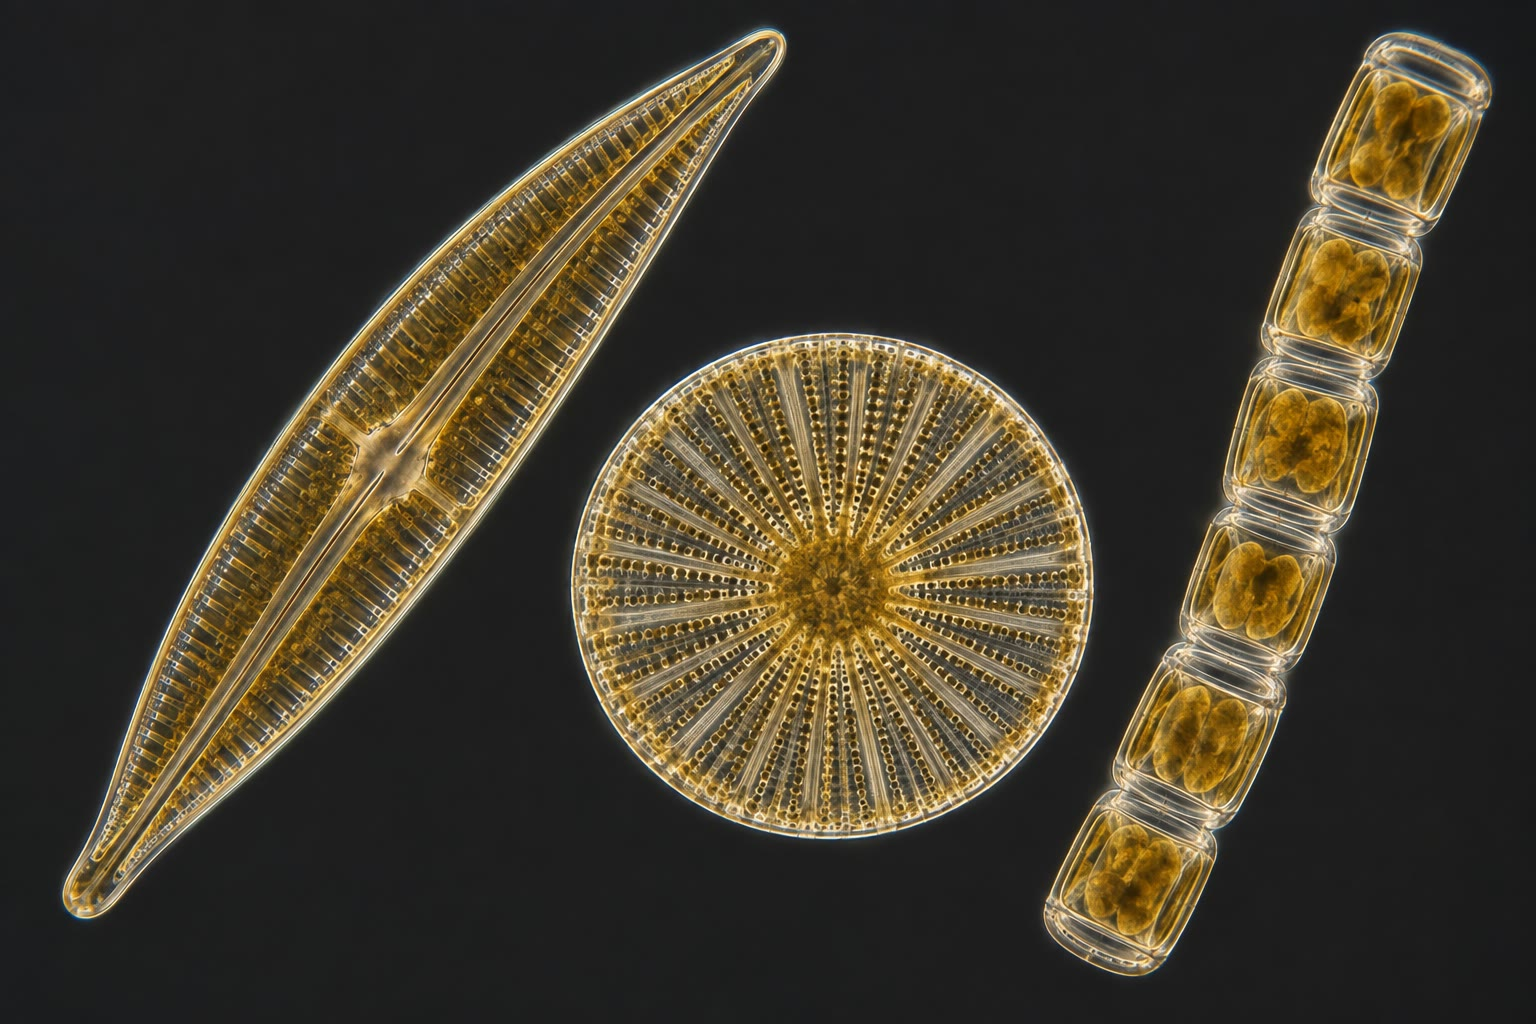
\includegraphics[width=0.6\linewidth]{images/book4/ai/b4-01-diatoms.jpg}

{\small Diatomeas vistas en microscopía de campo oscuro: cada célula vive
en un caparazón de sílice de dos valvas, surcado de poros a través de los
cuales intercambia con el agua.}
\end{omfigure}

\begin{definition}[Modos de nutrición]\label{def:b2:unicellular-diversity:nutrition}
\index{fagotrofia}\index{osmotrofia}\index{mixotrofia}
Un eucariota \omterm{def:b2:unicellular-diversity:unicellular}{unicelular} se alimenta de una de tres maneras, o de dos a la
vez. \emph{Fototrofia}: tiene cloroplastos y fabrica su propia materia
orgánica a partir de la luz y el $\mathrm{CO_2}$ (algas verdes, diatomeas,
dinoflagelados). \emph{Fagotrofia}: engloba partículas --- bacterias,
otros \omterm{def:b2:unicellular-diversity:protist}{protistas} --- en una vacuola digestiva donde las enzimas
lisosómicas las digieren (amebas, ciliados, coanoflagelados).
\emph{Osmotrofia}: absorbe moléculas disueltas a través de su membrana, a
menudo tras secretar enzimas al exterior (levaduras, muchos parásitos).
Los \emph{mixótrofos}, como \emph{Euglena}, hacen la fotosíntesis a la
luz y comen en la oscuridad. Los \omterm{def:b2:unicellular-diversity:prokaryote}{procariotas} no pueden fagocitar: la
pared se lo impide, y por eso ningún \omterm{def:b2:unicellular-diversity:prokaryote}{procariota} llegó a ser un
depredador que engloba a sus presas.
\end{definition}

\begin{proposition}[Osmorregulación en agua dulce]\label{prop:b2:unicellular-diversity:osmoregulation}
\index{vacuola contráctil}
Un \omterm{def:b2:unicellular-diversity:protist}{protista} de agua dulce es mucho más salado por dentro (unos
\qty{100}{mmol/L} de solutos) que la charca (alrededor de
\qty{1}{mmol/L}), y su membrana deja pasar el agua. El agua entra por
tanto continuamente por ósmosis, a un ritmo proporcional a la superficie
y a la diferencia de presión osmótica $\Delta\Pi = RT\,\Delta c$ ---
unos \qty{2.4}{bar} para las cifras anteriores. Una célula con pared
resiste gracias a la turgencia; una célula desnuda se hincharía y
estallaría en pocos minutos. La \emph{\omterm{prop:b2:unicellular-diversity:osmoregulation}{vacuola contráctil}} es la
respuesta: un reservorio alimentado por canales radiales que se llena
de agua bombeada por transportadores impulsados por protones y después se
contrae, expulsando el agua por un poro, cada pocos segundos o cada pocos
minutos. Un \emph{Paramecium} evacúa su propio volumen de agua cada media
hora; sus parientes marinos, en un medio tan salado como ellos mismos,
no tienen \omterm{prop:b2:unicellular-diversity:osmoregulation}{vacuola contráctil}.
\end{proposition}

\section{La física de un nadador diminuto}

\begin{proposition}[La vida a bajo número de Reynolds]\label{prop:b2:unicellular-diversity:reynolds}
\index{número de Reynolds}
El \emph{\omterm{prop:b2:unicellular-diversity:reynolds}{número de Reynolds}} $Re = \rho v L/\eta$ compara las fuerzas de
inercia con las viscosas para un cuerpo de tamaño $L$ que se mueve a
velocidad $v$ en un fluido de densidad $\rho$ y viscosidad $\eta$. Para
un nadador humano vale alrededor de $10^6$; para \emph{Paramecium}
(\qty{200}{\micro m}, \qty{1}{mm/s}) es 0,2, y para una bacteria
$10^{-5}$. Por debajo de $Re \approx 1$ la inercia es irrelevante: una
célula que deja de batir se detiene en menos de un nanómetro, el agua se
comporta como un jarabe espeso y un movimiento recíproco (el mismo golpe
hacia delante y hacia atrás) no produce ningún desplazamiento neto. Por
eso los nadadores pequeños usan golpes no recíprocos: la hélice giratoria
del flagelo bacteriano, el batido asimétrico de un cilio (golpe efectivo
rígido, golpe de recuperación curvado), la braza de
\emph{Chlamydomonas}.
\end{proposition}

\begin{theorem}[Ley de Stokes y sedimentación]\label{thm:b2:unicellular-diversity:stokes}
\index{ley de Stokes}
Una esfera de radio $r$ y densidad $\rho_{\text{cél}}$ que se mueve
lentamente en un fluido de viscosidad $\eta$ sufre un arrastre
$F = 6\pi\eta r v$. Abandonada a sí misma en agua de densidad $\rho$, se
hunde a la velocidad límite
\[
v_s = \frac{2\,r^2\,(\rho_{\text{cél}} - \rho)\,g}{9\eta},
\]
proporcional al cuadrado de su radio: una célula diez veces mayor se
hunde cien veces más deprisa. Por eso el fitoplancton es pequeño, por
eso las diatomeas llevan espinas y gotitas de aceite, y por eso una
\emph{Chlamydomonas} que deja de nadar sale de la zona iluminada en unos
pocos días.
\end{theorem}
\begin{proof}
A la velocidad límite el arrastre equilibra el peso aparente (el peso
menos el empuje): $6\pi\eta r v_s = \tfrac{4}{3}\pi r^3
(\rho_{\text{cél}} - \rho) g$. Despejando $v_s$ se obtiene la fórmula.
La propia ley de arrastre se deduce en la serie de física para
$Re \ll 1$; aquí se toma como dada.
\end{proof}

\begin{example}[La caída de una diatomea]\label{ex:b2:unicellular-diversity:fall}
Una diatomea céntrica de radio \qty{10}{\micro m}, \qty{100}{kg/m^3}
más densa que el agua de mar ($\eta = \qty{1e-3}{Pa.s}$), se hunde a
$v_s = 2\times 10^{-10}\times 100\times 9.81/(9\times 10^{-3}) =
\qty{2.2e-5}{m/s}$, unos \qty{2}{m} al día: abandonaría la capa iluminada
de \qty{50}{m} en menos de un mes. Sus poblaciones sobreviven porque la
turbulencia remueve el agua, porque las gotitas de aceite y una baja
densidad reducen $\rho_{\text{cél}} - \rho$, y porque una célula que se
hunde y se divide por el camino deja descendientes que vuelven a ser
elevados.
\end{example}

\begin{omfigure}
\begin{tikzpicture}
\begin{axis}[
  width=0.8\linewidth, height=6.0cm,
  axis x line=bottom, axis y line=left,
  xmode=log, ymode=log,
  xmin=0.5, xmax=200, ymin=1e-3, ymax=1e4,
  xlabel={radio (\unit{\micro m})}, ylabel={velocidad de hundimiento (\unit{\micro m/s})},
  xlabel style={font=\small, at={(axis description cs:0.5,-0.1)}, anchor=north},
  ylabel style={font=\small},
  tick label style={font=\small},
  clip=false,
]
\addplot[very thick, omDef, domain=0.5:200, samples=40] {0.218*x^2};
\addplot[only marks, mark=*, mark size=1.8pt, omThm] coordinates {(1,0.218) (10,21.8) (100,2180)};
\node[font=\scriptsize, anchor=west] at (axis cs:1.15,0.218) {bacteria};
\node[font=\scriptsize, anchor=west] at (axis cs:11.5,21.8) {diatomea};
\node[font=\scriptsize, anchor=east] at (axis cs:85,2180) {protista grande};
\end{axis}
\end{tikzpicture}

{\small Velocidad de hundimiento de Stokes en función del radio, para
células \qty{100}{kg/m^3} más densas que el agua. La pendiente de 2 en
ejes logarítmicos es la ley en $r^2$: una bacteria se hunde un
centímetro al día; un \omterm{def:b2:unicellular-diversity:protist}{protista} grande, un par de metros por hora.}
\end{omfigure}

\section{Reproducción y sexo en una sola célula}

\begin{definition}[Modos de división]\label{def:b2:unicellular-diversity:division}
\index{fisión binaria}\index{gemación}\index{fisión múltiple}
Un \omterm{def:b2:unicellular-diversity:unicellular}{organismo unicelular} se reproduce dividiéndose. \emph{Fisión
binaria}: la célula crece hasta duplicar su tamaño y se parte en dos
hijas iguales (bacterias, \emph{Paramecium}, \emph{Amoeba}).
\emph{Gemación}: una hija pequeña crece a partir de la madre y se
desprende (levadura; la madre conserva una cicatriz y puede gemar unas
veinte veces). \emph{Fisión múltiple}: la célula crece mucho y después se
divide varias veces seguidas dentro de la pared materna y libera de una
vez 4, 8, 16 o más hijas (\emph{Chlamydomonas}, el parásito de la malaria
en un glóbulo rojo). En condiciones constantes el número de células
crece exponencialmente, $N(t) = N_0\,2^{t/T}$, con $T$ el
\emph{tiempo de generación}\index{tiempo de generación}: veinte minutos
para \emph{E.~coli} en medio rico, un día para muchas algas, una semana
para algunos ciliados. (El crecimiento en función del alimento se trata
en el \cref{ch:b2:microbial-metabolism}.)
\end{definition}

\begin{proposition}[Sexo sin reproducción: la conjugación en \emph{Paramecium}]\label{prop:b2:unicellular-diversity:conjugation}
\index{conjugación!ciliados}
Dos \emph{Paramecium} de tipos sexuales complementarios se unen por sus
caras orales. En cada uno, el micronúcleo diploide sufre meiosis y da
cuatro núcleos haploides, tres de los cuales degeneran; el superviviente
se divide por mitosis en un núcleo estacionario y otro migratorio, y las
dos células intercambian sus núcleos migratorios a través de la unión.
Cada célula fusiona entonces su núcleo estacionario con el que ha
recibido, y los dos compañeros se separan, cada uno con un nuevo
micronúcleo diploide del mismo genotipo que el de su pareja. El
macronúcleo antiguo se desintegra y se construye uno nuevo a partir del
nuevo micronúcleo. No se ha formado ninguna célula nueva: la conjugación
es mezcla genética --- meiosis y fecundación,
\cref{ch:b2:meiosis-heredity} --- desacoplada de la multiplicación.
La conjugación bacteriana, que transfiere un \omterm{def:b2:unicellular-diversity:prokaryote}{plásmido} en un solo sentido
de un donante a un receptor, es un proceso distinto con el mismo nombre
(\cref{ch:b2:genome-diversification}).
\end{proposition}

\begin{omfigure}
\begin{tikzpicture}[every node/.style={font=\scriptsize}]
  \foreach \i/\x in {0/0,1/3.6,2/7.2,3/10.8} {
    \draw[thick, fill=omProp!8] (\x,0.55) ellipse (1.0 and 0.5);
    \draw[thick, fill=omProp!8] (\x,-0.55) ellipse (1.0 and 0.5);
  }
  % stage 0: two cells, diploid micronuclei 2n
  \fill[omDef!90!black] (0,0.55) circle (0.12); \node[right] at (0.15,0.55) {$2n$};
  \fill[omDef!90!black] (0,-0.55) circle (0.12); \node[right] at (0.15,-0.55) {$2n$};
  \node[below, align=center] at (0,-1.15) {dos células se unen};
  % stage 1: meiosis, 4 haploid, 3 degenerate
  \foreach \dy in {0.55,-0.55} {
    \fill[omDef!90!black] (3.6-0.3,\dy+0.15) circle (0.08);
    \fill[gray!60] (3.6+0.1,\dy+0.2) circle (0.06);
    \fill[gray!60] (3.6+0.3,\dy-0.05) circle (0.06);
    \fill[gray!60] (3.6-0.1,\dy-0.25) circle (0.06);
  }
  \node[below, align=center] at (3.6,-1.15) {meiosis:\\4 núcleos haploides,\\tres degeneran};
  % stage 2: mitosis, exchange
  \foreach \dy in {0.55,-0.55} {
    \fill[omDef!90!black] (7.2-0.35,\dy) circle (0.08);
    \fill[omThm] (7.2+0.35,\dy) circle (0.08);
  }
  \draw[->, thick, omThm] (7.55,0.45) -- (7.55,-0.45);
  \draw[->, thick, omThm] (6.85,-0.45) -- (6.85,0.45);
  \node[below, align=center] at (7.2,-1.15) {mitosis; se\\intercambian los núcleos\\migratorios (rojo)};
  % stage 3: fusion 2n
  \fill[omDef!90!black] (10.8,0.55) circle (0.12); \node[right] at (10.95,0.55) {$2n$};
  \fill[omDef!90!black] (10.8,-0.55) circle (0.12); \node[right] at (10.95,-0.55) {$2n$};
  \node[below, align=center] at (10.8,-1.15) {fecundación:\\nuevos núcleos diploides\\idénticos; se separan};
  \foreach \x in {1.3,4.9,8.5} \draw[->, thick, gray] (\x,0) -- (\x+1.0,0);
\end{tikzpicture}

{\small Conjugación en \emph{Paramecium}. Dos células intercambian núcleos
haploides y se separan, cada una con un micronúcleo diploide
recombinado; el número de células no ha cambiado.}
\end{omfigure}

\section{Hacia la pluricelularidad}

\begin{proposition}[La serie volvocal]\label{prop:b2:unicellular-diversity:volvox}
\index{Volvox@\emph{Volvox}}\index{pluricelularidad, origen de la}
Entre las algas verdes, un linaje muestra en especies vivas los pasos que
llevan de una célula a un cuerpo. \emph{Chlamydomonas} vive sola.
\emph{Gonium} es una placa plana de 4 a 16 células idénticas que nadan
juntas. \emph{Pandorina} y \emph{Eudorina} son esferas huecas de 16 a 32
células, todavía iguales, cada una capaz de fundar una colonia nueva.
\emph{Pleodorina} tiene algunas células pequeñas que solo nadan y nunca
se dividen. \emph{Volvox} es una esfera de \num{500} a \num{50000}
pequeñas células somáticas, flageladas, que morirán con la colonia,
alrededor de un puñado de grandes células germinales (gonidios) que se
dividen para formar esferas hijas dentro de la madre. Han aparecido
células somáticas y germinales: es el umbral de la pluricelularidad,
cruzado en este linaje hace unos \num{200} millones de años y, de forma
independiente, al menos veinticinco veces en otros puntos del árbol de
la vida --- en animales, plantas, hongos, algas pardas, algas rojas y
varios grupos bacterianos.
\end{proposition}
\begin{proof}[Evidencia]
La filogenia molecular de las algas volvocales, construida con decenas de
genes, sitúa a \emph{Chlamydomonas} en la base y a \emph{Volvox} en las
puntas, con las formas \omterm{def:b2:unicellular-diversity:unicellular}{coloniales} entre ambas y el número de células
creciendo a lo largo de las ramas; el genoma de \emph{Volvox carteri}
(2010) difiere del de \emph{Chlamydomonas} en unos pocos cientos de
genes, sobre todo los de la matriz extracelular que mantiene unidas las
células y los de los reguladores que silencian la división en las
células somáticas. La transición requirió notablemente poco material
genético nuevo.
\end{proof}

\begin{omfigure}
\begin{tikzpicture}[every node/.style={font=\scriptsize}]
  % Chlamydomonas
  \draw[thick, fill=omProp!25] (0,0) circle (0.22);
  \node[below=0.35cm, align=center] at (0,0) {\emph{Chlamydomonas}\\1 célula};
  % Gonium plate
  \begin{scope}[xshift=2.2cm]
    \foreach \x in {-0.3,0,0.3} \foreach \y in {-0.3,0,0.3} \draw[thick, fill=omProp!25] (\x,\y) circle (0.14);
    \draw[gray, dashed] (-0.55,-0.55) rectangle (0.55,0.55);
    \node[below=0.7cm, align=center] at (0,0) {\emph{Gonium}\\placa de 8--16};
  \end{scope}
  % Eudorina ball
  \begin{scope}[xshift=4.5cm]
    \draw[gray, dashed] (0,0) circle (0.6);
    \foreach \a in {0,45,...,315} \draw[thick, fill=omProp!25] (\a:0.55) circle (0.13);
    \draw[thick, fill=omProp!25] (0,0.1) circle (0.13);
    \node[below=0.7cm, align=center] at (0,0) {\emph{Eudorina}\\esfera de 32,\\todas iguales};
  \end{scope}
  % Pleodorina
  \begin{scope}[xshift=7.4cm]
    \draw[gray, dashed] (0,0) circle (0.7);
    \foreach \a in {0,30,...,330} \draw[thick, fill=omProp!25] (\a:0.62) circle (0.09);
    \foreach \a in {60,180,300} \draw[thick, fill=omProp!60] (\a:0.62) circle (0.14);
    \node[below=0.8cm, align=center] at (0,0) {\emph{Pleodorina}\\algunas células\\solo nadan};
  \end{scope}
  % Volvox
  \begin{scope}[xshift=10.6cm]
    \draw[thick, fill=omProp!6] (0,0) circle (0.95);
    \foreach \a in {0,12,...,348} \fill[omProp!70] (\a:0.9) circle (0.035);
    \foreach \a in {0,12,...,348} \fill[omProp!50] (\a:0.72) circle (0.03);
    \foreach \p in {(0.25,0.2),(-0.3,-0.25),(0.1,-0.4),(-0.2,0.35)} \draw[thick, omThm, fill=omThm!40] \p circle (0.13);
    \node[below=1.05cm, align=center] at (0,0) {\emph{Volvox}\\miles de células somáticas\\y unas pocas germinales (rojo)};
  \end{scope}
  \foreach \x in {0.5,3.0,5.3,8.3} \draw[->, gray] (\x,0) -- (\x+0.6,0);
\end{tikzpicture}

{\small La serie volvocal: una célula aislada, una placa, una esfera hueca
de células idénticas, una esfera en la que algunas células han renunciado
a dividirse, y \emph{Volvox}, donde miles de células somáticas mortales
rodean unas pocas células germinales.}
\end{omfigure}

\begin{omfigure}
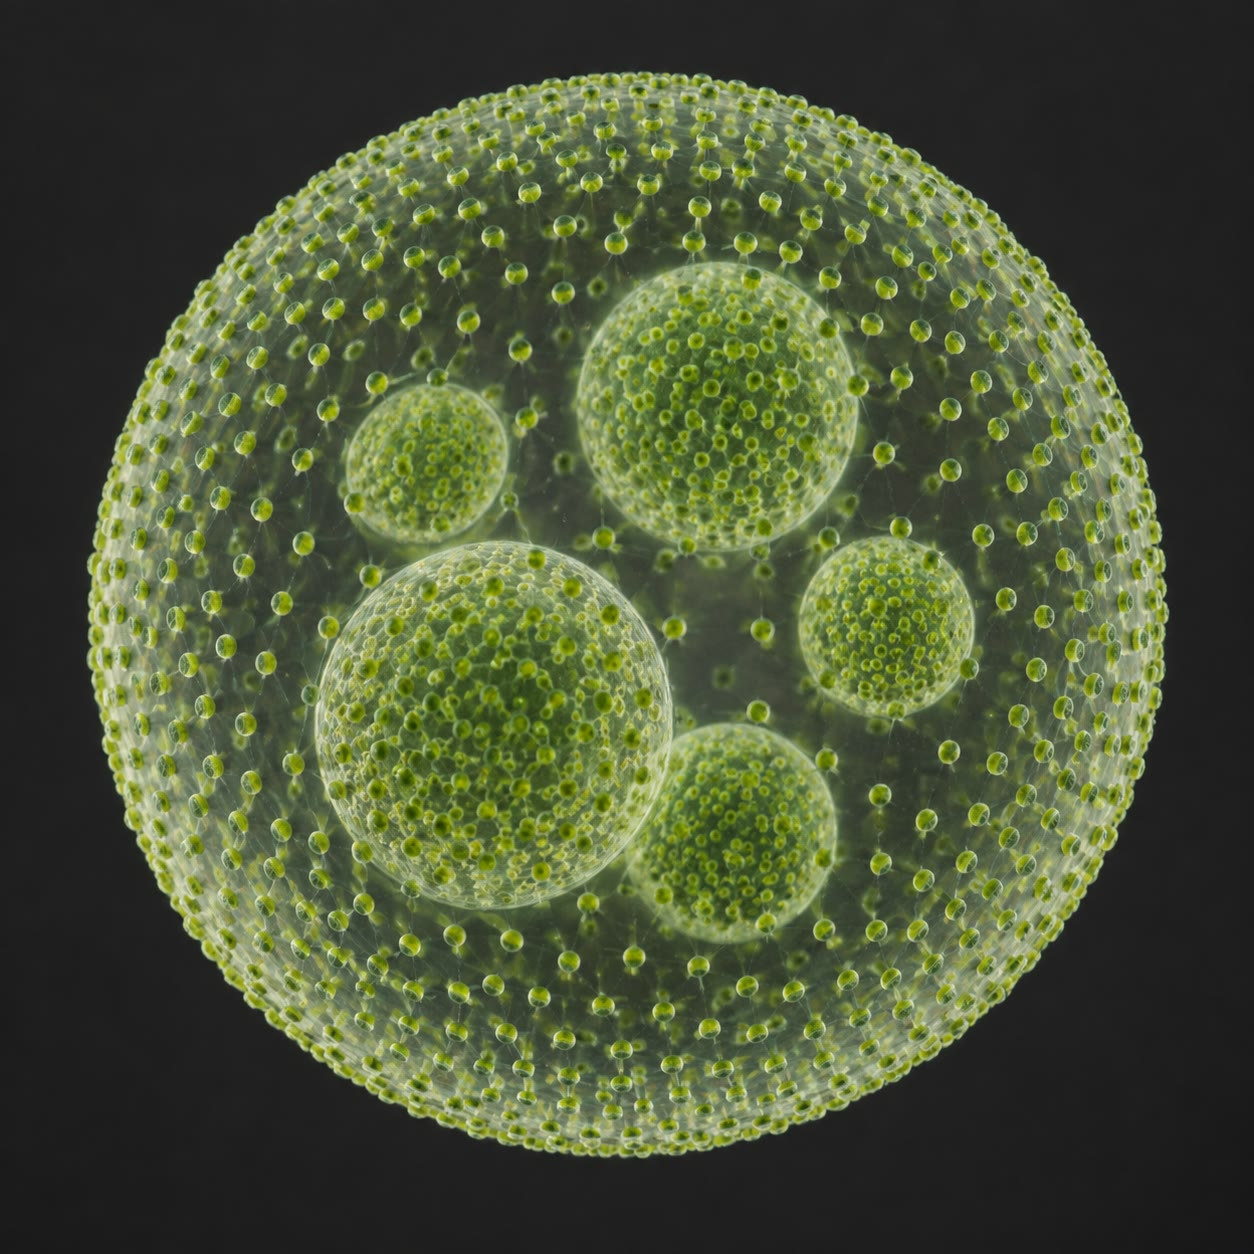
\includegraphics[width=0.55\linewidth]{images/book4/ai/b4-01-volvox.jpg}

{\small Una colonia de \emph{Volvox}: una esfera verde hueca de células
flageladas, con colonias hijas creciendo en su interior.}
\end{omfigure}

\begin{remark}[¿Por qué dividir el trabajo?]\label{rem:b2:unicellular-diversity:whydivide}
En estas algas una célula no puede nadar y dividirse a la vez: los
cuerpos basales que anclan los flagelos son necesarios para organizar el
huso. Una célula aislada alterna ambas tareas; una colonia pequeña puede
permitirse dejar de nadar mientras todas sus células se dividen; una
colonia grande se hundiría fuera de la luz (\omterm{thm:b2:unicellular-diversity:stokes}{ley de Stokes},
\cref{thm:b2:unicellular-diversity:stokes}) durante las horas que dura
su división. Por encima de cierto tamaño, mantener algunas células
nadando mientras otras se dividen compensa la pérdida de su descendencia
--- y nace un soma. Los coanoflagelados, flagelados con collar cuya
célula es una copia de la célula alimentadora de las esponjas, muestran
los mismos primeros pasos en la rama que condujo a los animales.
\end{remark}

\section{Ejercicios}

\begin{exercise}[$\star$]\label{exo:b2:unicellular-diversity:1}
Defínanse \omterm{def:b2:unicellular-diversity:unicellular}{unicelular}, \omterm{def:b2:unicellular-diversity:unicellular}{colonial} y \omterm{def:b2:unicellular-diversity:unicellular}{pluricelular}, y clasifíquense
\emph{E.~coli}, \emph{Gonium}, \emph{Volvox} y una célula de levadura en
la categoría correcta, justificando cada caso.
\end{exercise}

\begin{exercise}[$\star$]\label{exo:b2:unicellular-diversity:2}
Calcúlese la \omterm{prop:b2:unicellular-diversity:surface}{relación superficie/volumen} de un coco de radio
\qty{0.5}{\micro m} y de un \omterm{def:b2:unicellular-diversity:protist}{protista} esférico de radio
\qty{50}{\micro m}. ¿Cuál respira más deprisa por unidad de citoplasma,
y por qué?
\end{exercise}

\begin{exercise}[$\star$]\label{exo:b2:unicellular-diversity:3}
Dense tres diferencias estructurales entre una bacteria y un eucariota
\omterm{def:b2:unicellular-diversity:unicellular}{unicelular}, y una cosa que una ameba puede hacer y una bacteria no.
\end{exercise}

\begin{exercise}[$\star$]\label{exo:b2:unicellular-diversity:4}
Indíquese la función de cada una de las siguientes estructuras de
\emph{Paramecium}: cilios, surco oral, vacuola digestiva, \omterm{prop:b2:unicellular-diversity:osmoregulation}{vacuola
contráctil}, macronúcleo, micronúcleo.
\end{exercise}

\begin{exercise}[$\star\star$]\label{exo:b2:unicellular-diversity:5}
Con $D = \qty{5e-10}{m^2/s}$ para un metabolito en el citoplasma, ¿cuánto
tarda la difusión en atravesar una bacteria de \qty{1}{\micro m} y una
ameba de \qty{500}{\micro m}? Coméntese qué debe hacer la ameba que la
bacteria no necesita hacer.
\end{exercise}

\begin{exercise}[$\star\star$]\label{exo:b2:unicellular-diversity:6}
Calcúlese el \omterm{prop:b2:unicellular-diversity:reynolds}{número de Reynolds} de un \emph{Paramecium} (\qty{200}{\micro
m}, \qty{1}{mm/s}), de una bacteria (\qty{2}{\micro m}, \qty{20}{\micro
m/s}) y de un nadador humano (\qty{2}{m}, \qty{1}{m/s}), con
$\rho = \qty{1000}{kg/m^3}$ y $\eta = \qty{1e-3}{Pa.s}$. ¿Por qué un
nadador puede deslizarse tras una brazada y una bacteria no?
\end{exercise}

\begin{exercise}[$\star\star$]\label{exo:b2:unicellular-diversity:7}
Una diatomea de radio \qty{10}{\micro m} es \qty{100}{kg/m^3} más densa
que el agua. Calcúlense su velocidad de hundimiento y el tiempo que
tarda en descender \qty{50}{m}. ¿En qué factor cambia ese tiempo si la
célula reduce su radio a la mitad? ¿Y si reduce su exceso de densidad a
\qty{20}{kg/m^3}?
\end{exercise}

\begin{exercise}[$\star\star$]\label{exo:b2:unicellular-diversity:8}
Modélese un \emph{Paramecium} como un elipsoide de semiejes \num{100},
\num{25} y \qty{25}{\micro m} ($V = \tfrac{4}{3}\pi abc$). Expulsa su
propio volumen de agua cada \qty{30}{min}. Calcúlese la entrada de agua
en \unit{\micro m^3/s} y en litros por segundo.
\end{exercise}

\begin{exercise}[$\star\star$]\label{exo:b2:unicellular-diversity:9}
Un atrayente duplica su concentración a lo largo de \qty{1}{mm}. ¿Cuál
es la diferencia relativa entre los dos extremos de una bacteria de
\qty{1}{\micro m}? ¿Y entre el principio y el final de una carrera de
\qty{1}{s} a \qty{20}{\micro m/s}? Contar $N$ moléculas tiene un error
relativo de alrededor de $1/\sqrt{N}$: explíquese por qué la bacteria
compara instantes y no lados.
\end{exercise}

\begin{exercise}[$\star\star\star$]\label{exo:b2:unicellular-diversity:10}
\emph{Thiomargarita namibiensis} es una bacteria del azufre esférica de
\qty{500}{\micro m} de diámetro cuyo citoplasma es una capa de
\qty{2}{\micro m} de espesor alrededor de una vacuola de nitrato.
Calcúlese la relación entre su superficie y su volumen
\emph{citoplasmático} y compárese con la de \emph{E.~coli} (un cilindro
de radio \qty{0.5}{\micro m}; despréciense los extremos). Explíquese cómo
la vacuola le permite ser tan grande y para qué sirve el nitrato.
\end{exercise}

\begin{exercise}[$\star\star\star$]\label{exo:b2:unicellular-diversity:11}
En \emph{Volvox} las células somáticas nunca se dividen y mueren con la
colonia. A partir de la restricción de la flagelación y de la \omterm{thm:b2:unicellular-diversity:stokes}{ley de
Stokes}, explíquese por qué tales células compensan en una colonia de
\num{10000} células pero no en una de 16, y por qué las células
germinales son las más grandes de la esfera.
\end{exercise}

\begin{exercise}[$\star\star\star$]\label{exo:b2:unicellular-diversity:12}
``\omterm{def:b2:unicellular-diversity:protist}{Protista} es un grado, no un clado.'' Explíquese la distinción con los
linajes citados en este capítulo, y dígase por qué la misma afirmación
es cierta para ``\omterm{def:b2:unicellular-diversity:prokaryote}{procariota}'' y falsa para ``cianobacteria''.
\end{exercise}

\section{Problema: una gota de agua de charca}

\begin{problem}[{Problema de fin de semana --- una muestra de agua de
charca se cuenta, se cultiva y se analiza según la física que gobierna sus
células, hasta llegar al balance de agua y de energía de un alga verde}]
\label{pb:b2:unicellular-diversity:1}
En primavera se toma una muestra de una charca de \qty{1000}{m^3}. Al
microscopio, una cámara de recuento cuya cuadrícula cubre
\qty{1}{mm}$\times$\qty{1}{mm}, bajo un cubreobjetos situado a
\qty{0.1}{mm} por encima, muestra 24 células de \emph{Chlamydomonas}
(esferas de radio \qty{5}{\micro m} y densidad \qty{1050}{kg/m^3}).
Tómense $\rho = \qty{1000}{kg/m^3}$,
$\eta = \qty{1e-3}{Pa.s}$, $g = \qty{9.81}{m/s^2}$, $R =
\qty{8.314}{J/mol/K}$, $T = \qty{293}{K}$, y $D = \qty{1.9e-9}{m^2/s}$
para el $\mathrm{CO_2}$ en agua.

\medskip
\noindent\textbf{Parte I --- Recuento.}
\begin{enumerate}
  \item Calcúlese el volumen de agua bajo la cuadrícula, en microlitros.
  \item Dedúzcase la densidad de \emph{Chlamydomonas} en la charca, en
        células por mililitro.
  \item Calcúlense el volumen y la \omterm{prop:b2:unicellular-diversity:surface}{relación superficie/volumen} de una
        célula.
  \item ¿Qué fracción del volumen de agua de la charca ocupan estas
        células?
  \item ¿Cuántas \emph{Chlamydomonas} contiene la charca?
  \item También hay una cianobacteria filamentosa. Dense dos rasgos
        visibles al microscopio que la distingan del alga.
\end{enumerate}

\medskip
\noindent\textbf{Parte II --- Crecimiento.}
La muestra se mantiene a la luz y se vuelve a contar al cabo de
\qty{48}{h}: \num{384} células bajo la cuadrícula.
\begin{enumerate}[resume]
  \item Calcúlese el \omterm{def:b2:unicellular-diversity:division}{tiempo de generación} $T$.
  \item Calcúlese la constante de crecimiento $k$ de $N = N_0 e^{kt}$, en
        \unit{h^{-1}}.
  \item ¿Cuánto tardaría la población de la charca en alcanzar
        \qty{1e8}{} células por mililitro a este ritmo?
  \item Dense tres razones por las que no lo hará.
  \item Si las células solo crecen durante las \qty{12}{h} de luz y nada
        durante la noche, ¿cuánto tarda el mismo aumento?
  \item \emph{Chlamydomonas} se divide por \omterm{def:b2:unicellular-diversity:division}{fisión múltiple} y libera de una
        vez 4, 8 o 16 hijas. Explíquese por qué el recuento define aun así
        un \omterm{def:b2:unicellular-diversity:division}{tiempo de generación}.
\end{enumerate}

\medskip
\noindent\textbf{Parte III --- La física de la célula.}
\begin{enumerate}[resume]
  \item Calcúlese el \omterm{prop:b2:unicellular-diversity:reynolds}{número de Reynolds} de una célula que nada a
        \qty{100}{\micro m/s}.
  \item Una célula de masa $m$ que deja de batir sus flagelos avanza por
        inercia una distancia $mv/(6\pi\eta r)$. Calcúlese.
  \item Calcúlese la velocidad de hundimiento de una célula que ha dejado
        de nadar.
  \item Compárese el tiempo que tarda en hundirse \qty{1}{m} con el que
        tarda en subir nadando \qty{1}{m}.
  \item La charca contiene \qty{10}{\micro mol/L} de $\mathrm{CO_2}$
        disuelto. Calcúlese el aporte difusivo máximo de
        $\mathrm{CO_2}$ a una célula, en moléculas por segundo.
  \item Una célula contiene \qty{100}{pg} de carbono y lo duplica en una
        generación. Calcúlense su demanda media de carbono en moléculas
        por segundo y la razón entre aporte y demanda.
  \item Rehágase la comparación para una célula hipotética de radio
        \qty{50}{\micro m} con la misma densidad de carbono. Conclúyase.
\end{enumerate}

\medskip
\noindent\textbf{Parte IV --- Agua y energía.}
El citoplasma contiene \qty{100}{mmol/L} de solutos; la charca,
\qty{1}{mmol/L}. La conductividad hidráulica de la membrana es $L_p =
\qty{1e-14}{m.s^{-1}.Pa^{-1}}$ (flujo de volumen de agua por unidad de
superficie y por unidad de diferencia de presión). La hidrólisis de un
ATP libera \qty{50}{kJ/mol}; fijar un átomo de carbono cuesta tres ATP.
\begin{enumerate}[resume]
  \item Calcúlese la diferencia de presión osmótica a través de la membrana.
  \item Calcúlese el volumen de agua que entra en la célula por segundo, en
        \unit{\micro m^3/s}.
  \item Sin \omterm{prop:b2:unicellular-diversity:osmoregulation}{vacuola contráctil}, ¿cuánto tardaría la célula en duplicar su
        volumen?
  \item Calcúlese la potencia mínima necesaria para expulsar esta agua
        contra la presión osmótica.
  \item Conviértase en moléculas de ATP por segundo y compárese con el ATP
        que la célula gasta en la fijación del carbono (pregunta 18).
  \item Enúnciese el resultado: la entrada de agua de la célula, el tiempo
        que tardaría en estallar y la fracción de su energía que le cuesta
        mantenerse a salvo del agua.
\end{enumerate}
\end{problem}
